\documentclass{article}

\usepackage{graphicx}
\graphicspath{ {.} }
\usepackage{float}
\usepackage{siunitx}
\usepackage{array}
\usepackage{multirow}
\usepackage[utf8]{inputenc}
\usepackage[T1]{fontenc}
\usepackage{polski}
\usepackage{amsmath}

\title{\textbf{Raport 2}}
\author{Julia Krempińska, Filip Miśkiewicz}
\date{Czerwiec 2024}

\begin{document}

\maketitle

\section{Wprowadzenie}
W tym raporcie skupimy się na testowaniu hipotez dla różnych parametrów oraz wyznaczymy prawdopodobieństwo popełnienia błędów I i II rodzaju, a także sprawdzimy moc przeprowadzanych testów. % nie wiem co tu można jeszcze dopisać

\section{Przypadek nieznanej średniej}
Z populacji generalnej o rozkładzie normalnym $N(\mu, 0.2)$ pobrano próbę o dłuści n. Zweryfikujemy prawdziwość hipotez alteratywnych przy założeniu hipotezy zerowej $H_{0}: \mu = 1.5$. 
\subsection{Hipoteza alternatywna $H_{1}:\mu\neq1.5$}
W celu zweryfikowania hipotezy zerowej ustalamy statystykę testową
\begin{equation}
Z = \frac{\overline{X}-\mu_{0}}{\sigma\sqrt{n}}
\end{equation}
Gdzie $\overline{X}$ to średnia arytmetyczna ze wszystkich wartości jakie przyjmują dane, $n=1000$ to długość próby, $\mu_{0}=1.5$, a $\sigma=0.2$. Test przeprowadzimy na poziomie istotności $\alpha=0.05$.\\
Zbiór krytyczny definiujemy jako przedział wartości statystyki $Z$, dla którego odrzucamy hipotezę zerową i oznaczamy jako $C$. Dla przypadku hipotezy alternatywnej $H_{1}:\mu\neq1.5$ zbiór krytyczny konstruujemy w następujący sposób
\begin{equation}
C = (-\infty, -z_{1-\frac{\alpha}{2}}]\cup [z_{1-\frac{\alpha}{2}}, \infty)
\end{equation}
Gdzie $z_{1-\frac{\alpha}{2}}$ to kwantyl rzędu $1-\frac{\alpha}{2}$ rozkładu $N(0,1)$.
Dla naszych danych obliczamy wartość statystyki $Z$. Zaczynamy od policzenia średniej wartości  
\begin{equation}
\overline{X} = \frac{1}{n}\sum_{i=1}^{n}X_{i} = \frac{1}{1000}\sum_{i=1}^{1000}X_{i} \approx1.456
\end{equation}
Teraz podstawiamy do wzoru na statystykę testową
\begin{equation}
Z = \frac{1,456-1.5}{0.2\cdot31.623} = -7.042
\end{equation}
Aby sprawdzić czy wartość naszej statystyki znajduje się w zbiorze krytycznym wyznaczamy wartość kwantyla rozkładu normalnego standardowego rzędu $0.975$. Otrzymujemy $z_{0.975}\approx1.960$. Wiemy stąd, że 
\begin{equation}
C = (-\infty,-1.960]\cup[1.960,\infty)
\end{equation}
Wyznaczony zbiór krytyczny jest przedstawiony poniżej
\begin{figure}[H]
    \centering
    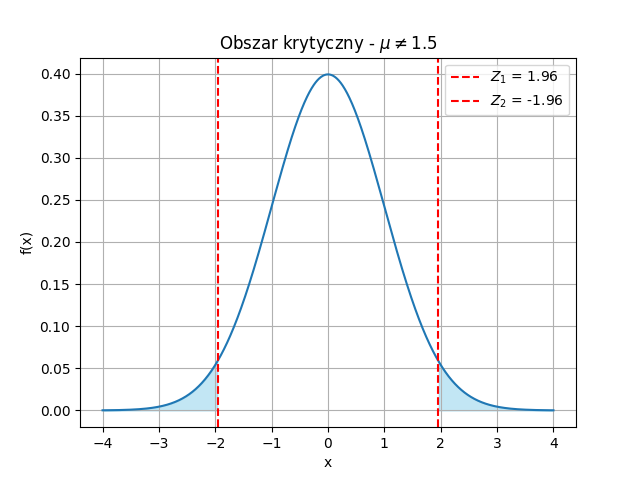
\includegraphics[scale=0.5]{mu_neq.png}
    \caption{Zbiór krytyczny dla hipotezy $H_{1}:\mu\neq1.5$}
    \label{fig:1}
\end{figure}

Zatem otrzymane wcześniej $Z$ zawiera się w zbiorze $C$ i mamy podstawy do odrzucenia hipotezy zerowej oraz przyjęcia hipotezy alternatywnej $H_{1}:\mu\neq1.5$.\\
Teraz wyznaczymy p-wartość. Jest to najmniejszy poziom istotności $\alpha$, przy którym zaobserwowana wartość statystyki prowadzi do odrzucenia hipotezy zerowej. Dla tej hipotezy alternatywnej p-wartość obliczamy ze wzoru
\begin{equation}
    p = 2(1-\Phi(|z|))
\end{equation}
gdzie $\Phi(x)$ to wartość dystrybuanty rozkładu normalnego standardowego w punkcie $x$.\\
Dla naszych danych p-wartość wynosi $p=1.9\times10^{-12}$. Oznacza to, że dla $\alpha<p$ przyjęlibyśmy hipotezę zerową.

\subsection{Hipoteza alternatywna $H_{1}: \mu>1.5$}
W celu zweryfikowania hipotezy zerowej ustalamy statystykę testową taką jak dla poprzedniej hipotezy alternatywnej. Dla przypadku hipotezy alternatywnej $H_{1}:\mu>1.5$ zbiór krytyczny konstruujemy w następujący sposób
\begin{equation}
C = [z_{1-\alpha}, \infty)
\end{equation}
Wartość statystyki testowej pozostaje bez zmian, czyli $Z=-7.042$. Aby sprawdzić czy wartość naszej statystyki znajduje się w zbiorze krytycznym wyznaczamy wartość kwantyla rozkładu normalnego standardowego rzędu $0.95$. Otrzymujemy $z_{0.95}\approx1.645$. Wiemy stąd, że 
\begin{equation}
C = [1.645,\infty)
\end{equation}
Wyznaczony zbiór krytyczny jest przedstawiony poniżej
\begin{figure}[H]
    \centering
    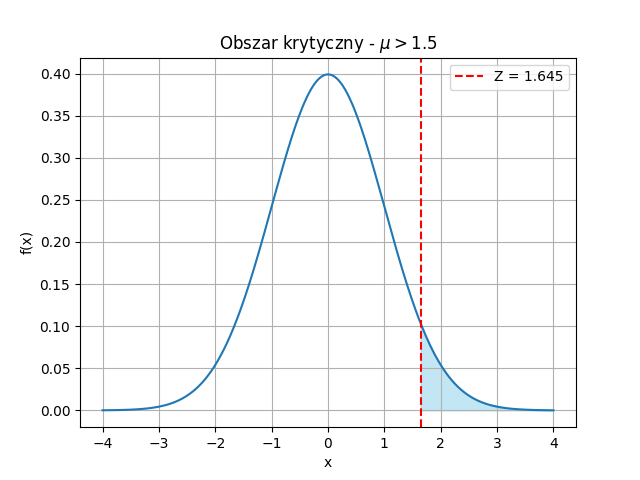
\includegraphics[scale=0.5]{mu_g.png}
    \caption{Zbiór krytyczny dla hipotezy $H_{1}:\mu>1.5$}
    \label{fig:2}
\end{figure}
Zatem otrzymane wcześniej $Z$ nie zawiera się w zbiorze $C$ i przyjmujemy hipotezę zerową oraz odrzucamy hipotezę alternatywną $H_{1}:\mu>1.5$.\\
Dla tej hipotezy alternatywnej p-wartość obliczamy ze wzoru
\begin{equation}
    p = 1-\Phi(Z)
\end{equation}
Dla naszych danych p-wartość wynosi $p=0.999\dots$. Oznacza to, że dla $\alpha>p$ odrzucilibyśmy hipotezę zerową.

\subsection{Hipoteza alternatywna $H_{1}: \mu<1.5$}
Postępujemy analogicznie jak w poprzednim przypadku . Zbiór krytyczny konstruujemy w następujący sposób
\begin{equation}
C = (-\infty, -z_{1-\alpha}]
\end{equation}
Wartość statystyki testowej pozostaje bez zmian, czyli $Z=-7.042$. Wiemy z poprzedniego przypadku, że $z_{0.95}\approx1.645$. Stąd mamy
\begin{equation}
C = (-\infty,-1.645]
\end{equation}
Wyznaczony zbiór krytyczny jest przedstawiony poniżej
\begin{figure}[H]
    \centering
    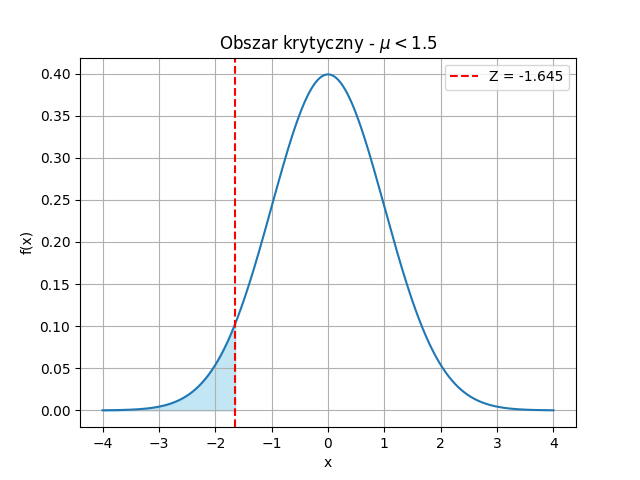
\includegraphics[scale=0.5]{mu_l.png}
    \caption{Zbiór krytyczny dla hipotezy $H_{1}:\mu<1.5$}
    \label{fig:3}
\end{figure}
Zatem otrzymane wcześniej $Z$ zawiera się w zbiorze $C$ i mamy podstawy do odrzucenia hipotezy zerowej oraz przyjęcia hipotezy alternatywnej $H_{1}:\mu<1.5$.\\
Dla tej hipotezy alternatywnej p-wartość obliczamy ze wzoru
\begin{equation}
    p = \Phi(Z)
\end{equation}
Dla naszych danych p-wartość wynosi $p=9.51\times10^{-13}$. Oznacza to, że dla $\alpha<p$ przyjęlibyśmy hipotezę zerową.

\subsection{Wnioski}
Z przeprowadzonych testów wynika, że $\mu<1.5$. Wartości p pozwalają założyć dużą istotność statystyczną przeprowadzonych testów. Po przetestowaniu na poziomach istotności $\alpha=0.1$ i $\alpha=0.01$ otrzymaliśmy takie same wyniki. 

\subsection{Kod w Pythonie}
Poniżej znajduje się kod napisany w języku Python rozwiązujący rozważany problem.
\begin{verbatim}
import numpy as np
from scipy.stats import norm
from urllib.request import urlopen
import matplotlib.pyplot as plt


url = "https://prac.im.pwr.edu.pl/~wyloman/ss_2023_2024/lista8_zad1.txt"
page = urlopen(url)
html_lines = page.readlines()
data = [float(line.decode("utf-8")) for line in html_lines]
np.array(data)

H0 = 1.5
sig = 0.2
n = len(data)
alpha = 0.05

data_mean = np.mean(data)
z = (data_mean - H0) / (sig / np.sqrt(n))
Z_quantile = norm.ppf(1 - (alpha/2))

# p-wartości
p_g = 1 - norm.cdf(z)
p_neq = 2 * (1 - norm.cdf(abs(z)))
p_l = norm.cdf(z)


# mu != 1.5 <- hipoteza alternatywna
if z <= -Z_quantile or z >= Z_quantile:
    print('Hipoteza mu != 1.5 prawdziwa')
else: 
    print('Hipoteza mu != 1.5 fałszywa')

Z_quantile = norm.ppf(1 - alpha)

# mu > 1.5 <- hipoteza alternatywna
if z > Z_quantile:
    print('Hipoteza mu > 1.5 prawdziwa')    
else:
    print('Hipoteza mu > 1.5 fałszywa')

# mu < 1.5 <- hipoteza alternatywna
if z < -Z_quantile:
    print('Hipoteza mu < 1.5 prawdziwa')    
else:
    print('Hipoteza mu < 1.5 fałszywa')
\end{verbatim}
Kod zwrócił następujące wyniki
\begin{verbatim}
Hipoteza mu != 1.5 prawdziwa
Hipoteza mu > 1.5 fałszywa
Hipoteza mu < 1.5 prawdziwa
\end{verbatim}


\section{Przypadek nieznanej wariancji}
Z populacji generalnej o rozkładzie normalnym $N(0.2, \sigma^{2}$ pobrano próbę o dłuści n. Zweryfikujemy prawdziwość hipotez alteratywnych przy założeniu hipotezy zerowej $H_{0}: \sigma^{2}= 1.5$.

\subsection{Hipoteza alternatywna $H_{1}:\sigma\neq1.5$}
W celu zweryfikowania hipotezy zerowej ustalamy statystykę testową
\begin{equation}
\chi = \frac{(n-1)s^{2}}{\sigma_{0}^{2}}
\end{equation}
gdzie $n=1000$ jest długością próby, $s^{2}$ to wariancja wyznaczona z próby, $\sigma_{0}^{2}=1.5$. Test przeprowadzimy na poziomie istotności $\alpha=0.05$.\\
Zbiór krytyczny definiujemy jako przedział wartości statystyki $\chi$, dla którego odrzucamy hipotezę zerową i oznaczamy jako $C$. Dla przypadku hipotezy alternatywnej $H_{1}:\sigma^{2}\neq1.5$ zbiór krytyczny konstruujemy w następujący sposób
\begin{equation}
C = (-\infty, x_{\frac{\alpha}{2},n-1}]\cup [x_{1-\frac{\alpha}{2},n-1}, \infty)
\end{equation}
Gdzie $x_{\frac{\alpha}{2},n-1}$ to kwantyl rzędu $\frac{\alpha}{2}$ rozkładu $\chi^{2}$ z $n-1$ stopniami swobody i analogicznie  $x_{1-\frac{\alpha}{2},n-1}$ to kwantyl rzędu $1-\frac{\alpha}{2}$ rozkładu $\chi^{2}$ z $n-1$ stopniami swobody .
Dla naszych danych obliczamy wartość statystyki $\chi$. Zaczynamy od policzenia wariancji ze wzoru
\begin{equation}
    s^{2}=\frac{1}{n}\sum^{n}_{i=1}(x_{i}-\overline{x})^{2}\approx1.667
\end{equation}
Teraz podstawiamy do wzoru na statystykę testową
\begin{equation}
    \chi=\frac{999\cdot1.667}{1.5}\approx1109.858
\end{equation}
Aby sprawdzić czy wartość naszej statystyki znajduje się w zbiorze krytycznym wyznaczamy wartość kwantyla rozkładu $\chi^{2}$ rzędu $0.025$ i $0.975$. Otrzymujemy $x_{0.025}\approx913.301$ i $x_{0.975}\approx1088.487$. Wiemy stąd, że 
\begin{equation}
C = (-\infty,913.301]\cup[1088.487,\infty)
\end{equation}
Wyznaczony zbiór krytyczny jest przedstawiony poniżej
\begin{figure}[H]
    \centering
    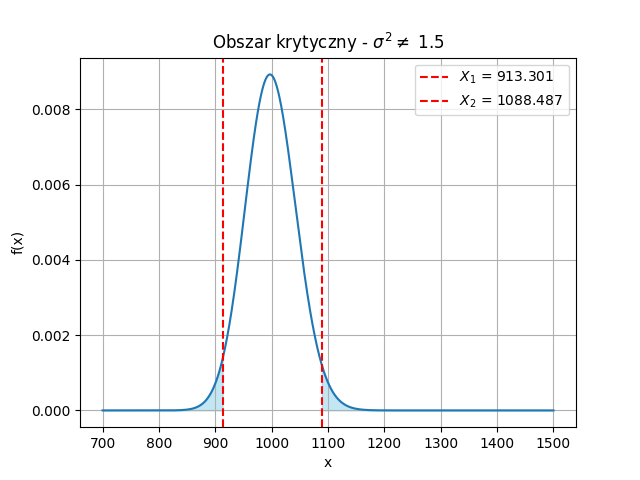
\includegraphics[scale=0.5]{sig_neq.png}
    \caption{Zbiór krytyczny dla hipotezy $H_{1}:\sigma^{2}\neq1.5$}
    \label{fig:4}
\end{figure}
Zatem otrzymane wcześniej $\chi$ zawiera się w zbiorze $C$ i mamy podstawy do odrzucenia hipotezy zerowej oraz przyjęcia hipotezy alternatywnej $H_{1}:\sigma^{2}\neq1.5$.\\
Teraz wyznaczymy p-wartość ze wzoru
\begin{equation}
    p = 2min(1-F_{\chi,n-1}(x), F_{\chi,n-1}(x))
\end{equation}
gdzie $F_{\chi,n-1}(x)$ to dystrybuanta rozkładu $\chi$ z $n-1$ stopniami swobody w punkcie $x$.\\
Dla naszych danych p-wartość wynosi $p=0.016$. Oznacza to, że dla $\alpha<p$ przyjęlibyśmy hipotezę zerową.

\subsection{Hipoteza alternatywna $H_{1}:\sigma^{2}>1.5$}
W celu zweryfikowania hipotezy zerowej ustalamy statystykę testową taką jak dla poprzedniej hipotezy alternatywnej. Dla przypadku hipotezy alternatywnej $H_{1}:\sigma^{2}>1.5$ zbiór krytyczny konstruujemy w następujący sposób
\begin{equation}
C = [x_{1-\alpha,n-1}, \infty)
\end{equation}
Wartość statystyki testowej pozostaje bez zmian, czyli $\chi=1109.858$. Aby sprawdzić czy wartość naszej statystyki znajduje się w zbiorze krytycznym wyznaczamy wartość kwantyla rozkładu $\chi^{2}$ rzędu $0.95$. Otrzymujemy $x_{0.95}\approx1073.643$. Wiemy stąd, że 
\begin{equation}
C = [1073.643,\infty)
\end{equation}
Wyznaczony zbiór krytyczny jest przedstawiony poniżej
\begin{figure}[H]
    \centering
    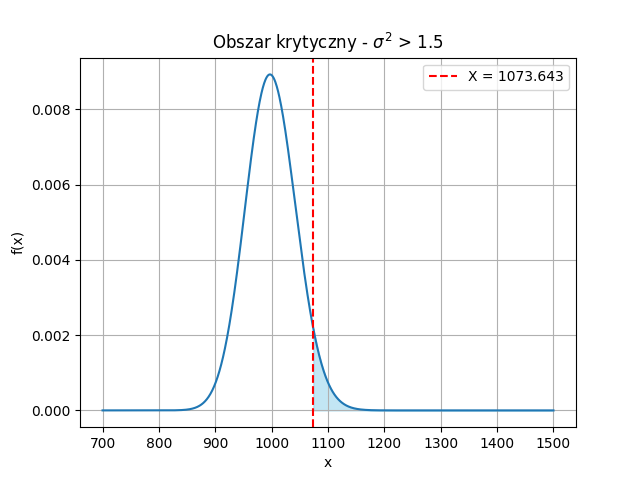
\includegraphics[scale=0.5]{sig_g.png}
    \caption{Zbiór krytyczny dla hipotezy $H_{1}:\sigma^{2}>1.5$}
    \label{fig:5}
\end{figure}
Zatem otrzymane wcześniej $\chi$ awiera się w zbiorze $C$ i mamy podstawy do odrzucenia hipotezy zerowej oraz przyjęcia hipotezy alternatywnej $H_{1}:\sigma^{2}>1.5$.\\
Dla tej hipotezy alternatywnej p-wartość obliczamy ze wzoru
\begin{equation}
    p = 1-F_{\chi,n-1}(x)
\end{equation}
Dla naszych danych p-wartość wynosi $p=0.008$. Oznacza to, że dla $\alpha<p$ przyjęlibyśmy hipotezę zerową.

\subsection{Hipoteza alternatywna $H_{1}: \sigma^{2}<1.5$}
Postępujemy analogicznie jak w poprzednim przypadku . Zbiór krytyczny konstruujemy w następujący sposób
\begin{equation}
C = (-\infty, x_{\alpha,n-1}]
\end{equation}
Wartość statystyki testowej pozostaje bez zmian, czyli $\chi=1109.858$. Aby sprawdzić czy wartość naszej statystyki znajduje się w zbiorze krytycznym wyznaczamy wartość kwantyla rozkładu $\chi^{2}$ rzędu $0.05$. Otrzymujemy $x_{0.05}\approx926.631$. Wiemy stąd, że 
\begin{equation}
C = (-\infty,926.631]
\end{equation}
Wyznaczony zbiór krytyczny jest przedstawiony poniżej
\begin{figure}[H]
    \centering
    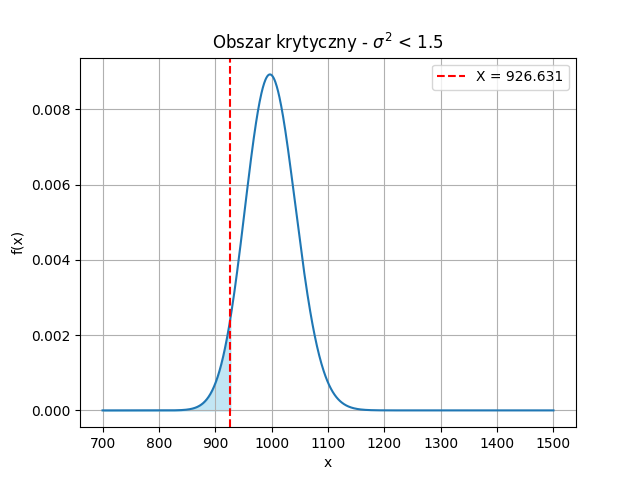
\includegraphics[scale=0.5]{sig_l.png}
    \caption{Zbiór krytyczny dla hipotezy $H_{1}:\sigma^{2}<1.5$}
    \label{fig:6}
\end{figure}
Zatem otrzymane wcześniej $\chi$ nie zawiera się w zbiorze $C$ i przyjmujemy hipotezę zerową oraz odrzucamy hipotezę alternatywną $H_{1}:\sigma^{2}<1.5$.\\
Dla tej hipotezy alternatywnej p-wartość obliczamy ze wzoru
\begin{equation}
    p = F_{\chi,n-1}(x)
\end{equation}
Dla naszych danych p-wartość wynosi $p=0.992$. Oznacza to, że dla $\alpha>p$ odrzucilibyśmy hipotezę zerową.

\subsection{Wnioski}
Z przeprowadzonych testów wynika, że $\sigma^{2}>1.5$. Wartości p pozwalają założyć dużą istotność statystyczną przeprowadzonych testów. Po przetestowaniu na poziomie istotności $\alpha=0.1$ otrzymaliśmy takie same wyniki, ale dla $\alpha=0.01$ należałoby przyjąć hipotezę zerową w przypadku $\sigma^{2}\neq1.5$ oraz $\sigma^{2}<1.5$.

\subsection{Kod w Pythonie}
Poniżej znajduje się kod napisany w języku Python rozwiązujący rozważany problem.
\begin{verbatim}
import numpy as np
from scipy.stats import chi2
from urllib.request import urlopen
import matplotlib.pyplot as plt


url = "https://prac.im.pwr.edu.pl/~wyloman/ss_2023_2024/lista8_zad2.txt"
page = urlopen(url)
html_lines = page.readlines()
data = [float(line.decode("utf-8")) for line in html_lines]
np.array(data)

H0 = 1.5
mu = 0.2
n = len(data)
alpha = 0.05

data_std = np.std(data)
x = ((n-1) * (data_std) ** 2) / H0 

X_quantile_low = chi2.ppf(alpha/2, n-1)
X_quantile_high = chi2.ppf(1 - (alpha/2), n-1)

# p-wartości
p_neq = 2 * min(1 - chi2.cdf(x, n-1), chi2.cdf(x, n-1))
p_g = 1 - chi2.cdf(x, n-1)
p_l = chi2.cdf(x, n-1)

# sig2 != 1.5 <- hipoteza alternatywna
if x <= X_quantile_low or x >= X_quantile_high:
    print('Hipoteza sig != 1.5 prawdziwa')
else: 
    print('Hipoteza sig != 1.5 fałszywa')

X_quantile = chi2.ppf(1 - alpha, n-1)

# sig > 1.5 <- hipoteza alternatywna
if x > X_quantile:
    print('Hipoteza sig > 1.5 prawdziwa')    
else:
    print('Hipoteza sig > 1.5 fałszywa')

X_quantile = chi2.ppf(alpha, n-1)

# sig < 1.5 <- hipoteza alternatywna
if x < X_quantile:
    print('Hipoteza sig < 1.5 prawdziwa')    
else:
    print('Hipoteza sig < 1.5 fałszywa')
\end{verbatim}
Kod zwrócił następujące wyniki
\begin{verbatim}
Hipoteza sig != 1.5 prawdziwa
Hipoteza sig > 1.5 prawdziwa
Hipoteza sig < 1.5 fałszywa
\end{verbatim}

%%%Tutaj zaczynam dodawać część do punktu o symulacyjnym prawdopodobieństwie błędów i mocach testu, więc jak coś się wysypie, to wywalić od tego momentu XD nie wiem czy to chcemy wkleić w środek do tych hipotez, czy ten podpunkt oddzielnie na koniec, ale wolę napisać w oddzielnej sekcji i potem najwyżej się poprzenosi żeby było składnie

\section{Wyznaczenie prawdopodobieństwa błędów}
Za pomocą Pythona możemy symulacyjne wyznaczyć prawdopodobieństwa wystąpienia błędów I i II rodzaju dla rozpatrywanych testów. Rozpoczniemy od wyznaczenia prawdopodobieństw błędu I rodzaju, zaczynając dla średniej i następnie dla wariancji, dla odpowiednich wartosci $\alpha$. Błąd pierwszego rodzaju wyznaczymy poprzez tysiąckrotne wygenerowanie próby losowej
z odpowiedniego rozkładu (standardowego normalnego lub chi2). Po przeprowdzeniu symulacji, możemy łatwo policzyć stosunek liczby prób w których statystyka testowa znajduje sie w obszarze krytycznym do liczby wszystkich prób. Operację powtórzymy stukrotnie  w celu uzyskania średniej wartości błedu. Obliczymy również medianę oraz odchylenie standardowe.
\subsection{Błąd I rodzaju}
\subsubsection{Populacja o rozkładzie o normalnym $N(\mu, 0.2)$}
Kod, który służy do wyznaczenia błędu I rodzaju dla $$H_1: \mu \neq 1.5, \alpha = 0.05:$$
\begin{verbatim}
import numpy as np
from scipy.stats import norm
import seaborn as sns
sns.set_style('whitegrid')
import matplotlib.pyplot as plt

alpha = 0.05
n = 1000       # długość pojedynczej próby
N = 1000       # liczba iteracji do symulacyjego wyznaczenia błędu I rodzaju
M = 100        # liczba wysymulowanych błędów I rodzaju 
mu = 1.5
sigma = 0.2

def critical_values(alpha):
    return norm.ppf(alpha/2), norm.ppf(1 - alpha/2)

def simulate_type1_error(alpha=alpha, mu=mu, sigma=sigma, n=n, N=N, M=M):
    type1_errors = []
    for _ in range(M):
        rejections = 0
        c1, c2 = critical_values(alpha)
        for _ in range(N):
            X = norm.rvs(loc=mu, scale=sigma, size=n)  # parametry zgodne z H0
            m = np.mean(X)
            Z = (m - mu) / (sigma / np.sqrt(n))  # statystyka testowa
            if not (c1 < Z < c2):  # Z w obszarze krytycznym?
                rejections += 1
        type1_errors.append(rejections/N)
    return type1_errors

type1_error = simulate_type1_error(alpha=alpha, mu=mu, sigma=sigma, n=n, N=N, M=M)
print("Średnia: ", np.mean(type1_error), ", Mediana: ",
np.median(type1_error), ", Odchylenie standardowe: ", np.std(type1_error))

fig, (ax_box, ax_hist) = plt.subplots(2, sharex=True, 
gridspec_kw={"height_ratios": (.15, .85)}, figsize=(15, 7))
sns.boxplot(x=type1_error, ax=ax_box, color="indigo")
sns.histplot(data=type1_error, ax=ax_hist, color="indigo")
ax_box.set(xlabel='')
plt.suptitle(f'Symulacyjny rozkład błędu pierwszego rodzaju ($H_1 \; \colon \; 
\mu \\neq 1.5, \; \\alpha = {alpha}$, N = {N}, M={M})', fontsize=20);
plt.axvline(x=alpha, linestyle='dashed')

\end{verbatim}
Powyższy kod zwrócił wykres przedstawiony na Rysunku~7 oraz wartości: \\
Średnia:  0.04991 , Mediana:  0.049 , Odchylenie standardowe:  0.00695427206830449
\begin{figure}[H]
    \centering
    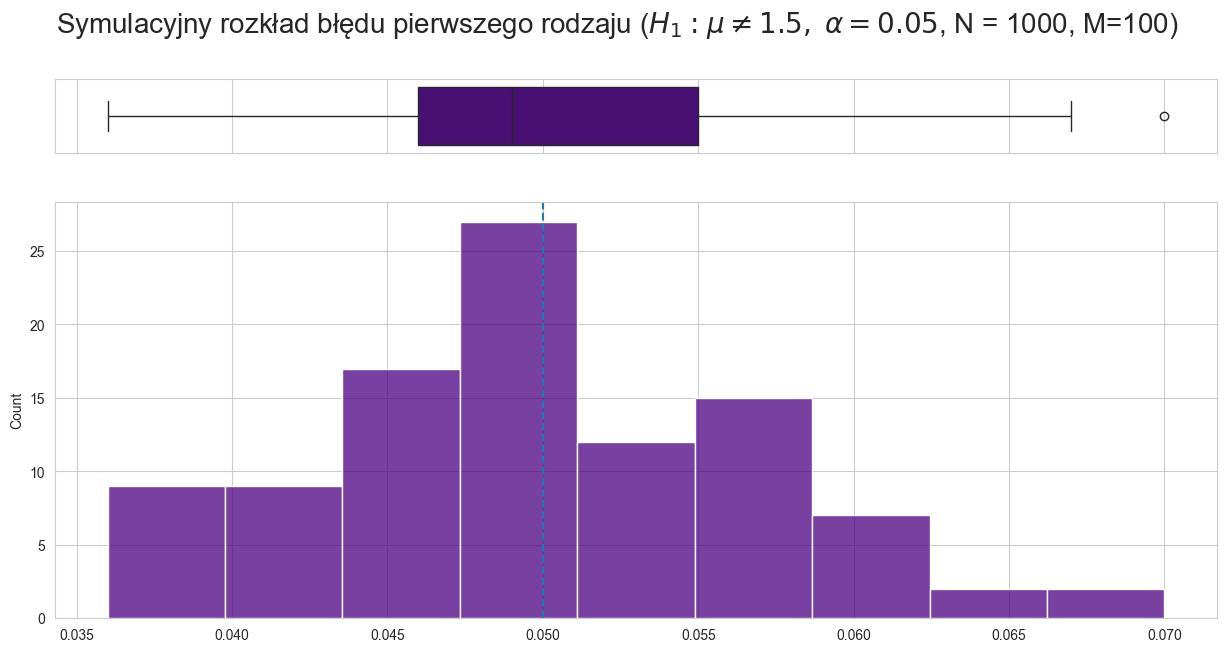
\includegraphics[scale=0.42]{22.png}
    \caption{Błąd pierwszego rodzaju jest bliski teoretycznej wartości poziomu istotności testu.}
    \label{fig:6}
\end{figure}
Za pomocą analogicznego kodu dla pozostałych wartości $\alpha$ oraz hipotez, otrzymujemy wartości, które umieszczone zostały w tabeli.
\begin{figure}[H]
    \centering
    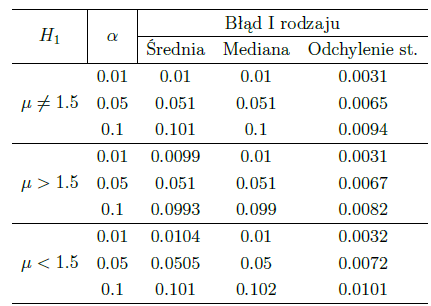
\includegraphics[scale=0.65]{tabelka_srednia1.png}
    \caption{Tabela przedstawia otrzymane rezultaty dla poszczególnych hipotez oraz różnych wartości $\alpha$.}
    \label{fig:6}
\end{figure}



\subsubsection{Populacja o rozkładzie normalnym $N(0.2, \sigma^2)$}
Kod potrzebny do wyznaczenia prawdopodobieństwa błędu I rodzaju w tym przypadku jest analogiczny jak dla pierwszego rozkładu, należy jednak pamiętać o podstawieniu rozkładu $\chi^2$ oraz zastosowaniu odpowiedniej statystyki testowej. W wyniku przeprowadzonych symulacji, otrzymujemy wartości przedstawione w tabeli (Rysunek~9).

\subsubsection{Wnioski}
Obserwujemy, że dla każdej z wartości, błąd pierwszego rodzaju jest zbliżony do poziomu istotności testu, zatem uzyskane wyniki symulacyjne należy uznać za poprawne.

\begin{figure}[H]
    \centering
    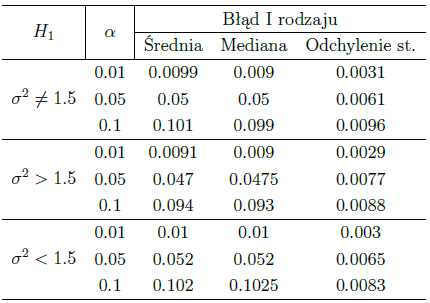
\includegraphics[scale=0.65]{tabelka_var1.png}
    \caption{Tabela przedstawia otrzymane rezultaty dla poszczególnych hipotez oraz różnych wartości $\alpha$.}
    \label{fig:6}
\end{figure}
\subsection{Błąd II rodzaju}
\subsubsection{Populacja o rozkładzie o normalnym $N(\mu, 0.2)$}
Kod, który służy do wyznaczenia błędu II rodzaju dla
$$H_1: \mu \neq 1.5, \alpha = 0.05:$$
\begin{verbatim}
import numpy as np
from scipy.stats import norm
import seaborn as sns
sns.set_style('whitegrid')
import matplotlib.pyplot as plt

mu0 = 1.5
#-----------
mu1 = 1.47
mu2 = 1.48
mu3 = 1.49
mu4 = 1.51
mu5 = 1.52
mu6 = 1.53
mus = [mu1, mu2, mu3, mu4, mu5, mu6]
alpha = 0.05
sigma = 0.2
n = 1000
N = 1000
M = 100
def critical_values(alpha):
    return norm.ppf(alpha/2), norm.ppf(1 - alpha/2)
def simulate_type2_error(alpha=alpha, mu=mu, mu0=mu0, sigma=sigma, 
n=n, N=N, M=M):
    type2_errors = []
    for _ in range(M):
        acceptances = 0
        c1, c2 = critical_values(alpha)
        for _ in range(N):
            X = norm.rvs(loc=mu, scale=sigma, size=n)  # parametry zgodne z H0
            m = np.mean(X)
            Z = (m - mu0) / (sigma / np.sqrt(n))  # statystyka testowa
            if (c1 < Z < c2):  # Z poza obszarem krytycznym?
                acceptances += 1
        type2_errors.append(acceptances/N)
    return type2_errors
for mu in mus:
    type2_error = simulate_type2_error(alpha=alpha, mu=mu, 
    sigma=sigma, n=n, N=N, M=M)
    print("Średnia: ", np.mean(type2_error), ",
    Mediana: ", np.median(type2_error), ",
    Odchylenie standardowe: ", np.std(type2_error))

    fig, (ax_box, ax_hist) = plt.subplots(2, sharex=True,
    gridspec_kw={"height_ratios": (.15, .85)}, figsize=(15, 7))
    sns.boxplot(x=type2_error, ax=ax_box, color="#0BCE9D")
    sns.histplot(data=type2_error, ax=ax_hist, color="#0BCE9D")
    ax_box.set(xlabel='')
    plt.suptitle(f'Symulacyjny rozkład błędu drugiego rodzaju ($H_1 \;
    colon \; \mu \\neq 1.5, \; \\alpha = {alpha}, \; \\mu = {mu}$,
    N = {N}, M={M})', fontsize=17);
    fig.savefig(f"box2_H1neq_{alpha}_{mu}.pdf")
\end{verbatim}
Powyższy kod zwraca kilka wykresów oraz wartości w zależności od parametru $\mu$. Przykładowy wykres dla $\mu = 1.51$ przedstawiony został na Rysunku~10. Analogicznie prezentuje się to dla pozostałych hipotez. Za pomocą otrzymanych wartości możemy wyznaczyć moc testu, którą definiujemy wzorem $$1 - P(B_{II}),$$ gdzie $P(B_{II})$ to prawdopodobieństwo błędu II rodzaju. Uzyskane wartości zostały przedstawione w tabeli na Rysunku~11.
\begin{figure}[H]
    \centering
    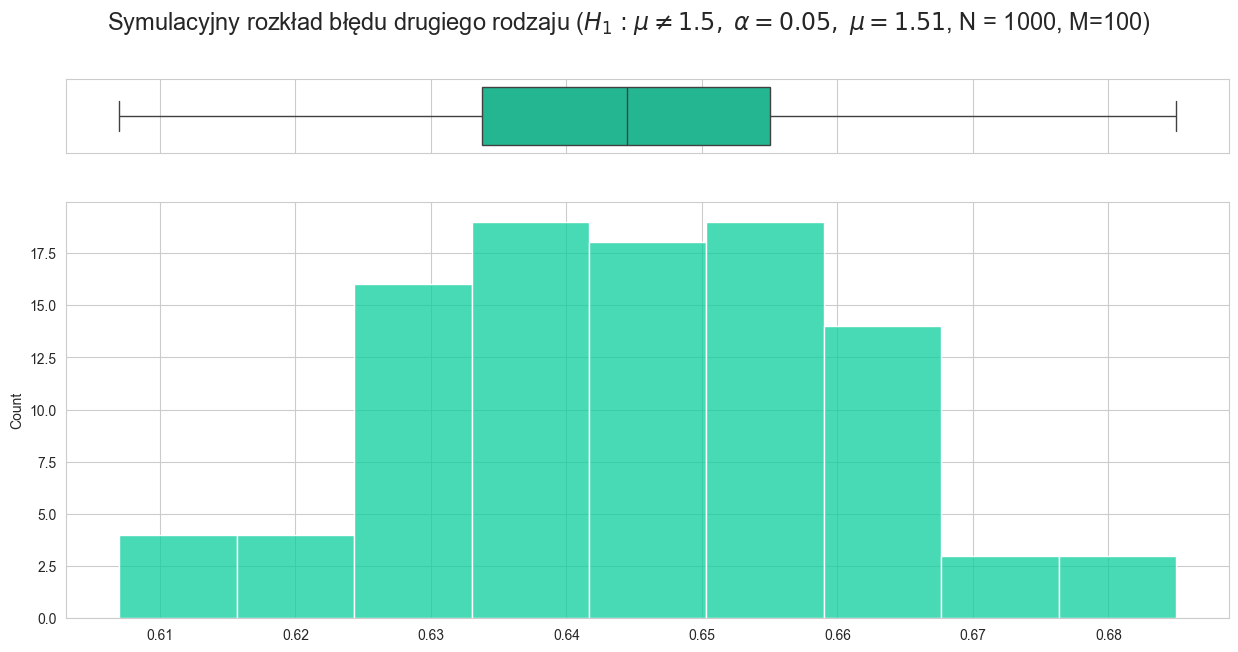
\includegraphics[scale=0.42]{mu151.png}
    \caption{Przykładowy wykres dla błędu II rodzaju.}
    \label{fig:6}
\end{figure}
\begin{figure}[H]
    \centering
    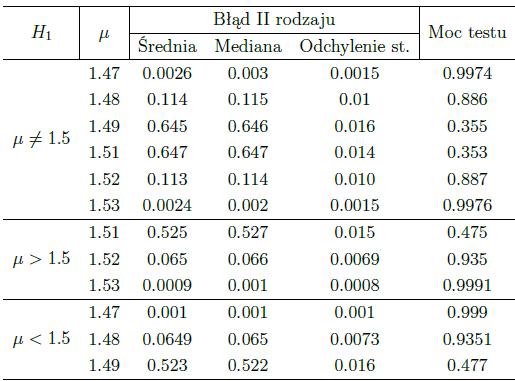
\includegraphics[scale=0.65]{tabelka_srednia2.png}
    \caption{Tabela przedstawia otrzymane rezultaty dla poszczególnych hipotez oraz różnych wartości $\mu$.}
    \label{fig:6}
\end{figure}
\subsection{Populacja o rozkładzie normalnym $N(0.2, \sigma^2)$}
Tę samą procedurę (z uwzględnieniem wymaganych zmian parametrów) stosujemy dla rozkładu $N(0.2, \sigma^2)$. Otrzymane wyniki przedstawione zostały w tabeli na Rysunku~12.
\begin{figure}[H]
    \centering
    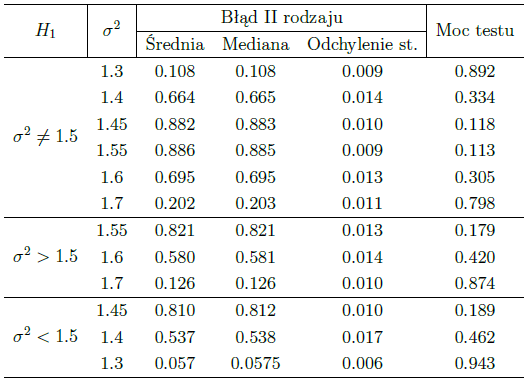
\includegraphics[scale=0.65]{tabelka_var2.png}
    \caption{Tabela przedstawia otrzymane rezultaty dla poszczególnych hipotez oraz różnych wartości $\sigma^2$.}
    \label{fig:6}
\end{figure}
\subsubsection{Wnioski}
Zarówno dla testu wariancji jak i testu średniej, obserwujemy, że im blizej
wartosci o której mówi hipoteza zerowa, tym wieksze prawdopodobienstwo błędu II rodzaju
i mniejsza moc testu. Dzieje się tak niezaleznie od wybranej hipotezy alternatywnej.
\end{document}





